\documentclass[aspectratio=169,10pt]{beamer}

% Version condensée de slides.tex : uniquement les résultats et les propositions.
% Mêmes figures (presentation/figures/), même style.

% ---------- Paquets ----------
\usefonttheme{professionalfonts}
\usepackage{fontspec}
\usepackage[french]{babel}
\usepackage{amsmath,amssymb}
\usepackage{booktabs}
\usepackage{array}
\usepackage{graphicx}
\graphicspath{{figures/}}

% ---------- Style ----------
\definecolor{bleu}{HTML}{1F4E79}
\definecolor{orange}{HTML}{E07B39}
\definecolor{vert}{HTML}{2E8B57}
\definecolor{rouge}{HTML}{C0392B}
\setbeamercolor{structure}{fg=bleu}
\setbeamercolor{frametitle}{fg=bleu}
\setbeamerfont{frametitle}{series=\bfseries,size=\Large}
\setbeamercolor{retenir}{bg=bleu!8,fg=black}
\setbeamertemplate{navigation symbols}{}
\setbeamertemplate{itemize items}[circle]
\setbeamertemplate{footline}{%
  \leavevmode\hbox to\paperwidth{\hspace{1.2em}\color{gray}\scriptsize\insertsectionhead\hfill
  \insertframenumber{} / \inserttotalframenumber\hspace{1.2em}}\vspace{0.7em}}

% Encadré « À retenir »
\newcommand{\retenir}[1]{\vfill\begin{beamercolorbox}[sep=5pt,rounded=true]{retenir}\small\textbf{Élément clé :} #1\end{beamercolorbox}}
\newcommand{\Qdix}{Q\textsubscript{10}}

\title{Spatialisation du \Qdix{} pour les modèles de surface terrestre}
\subtitle{Synthèse des résultats}
\author{Yassine Erraji \and William Peltier \and Simon Amar}
\date{Octobre 2026}

\begin{document}

% =====================================================================
\begin{frame}[plain]
  \titlepage
\end{frame}

% =====================================================================
\section{Contexte}

\begin{frame}{Le problème}
  \begin{itemize}
    \item Le \Qdix{} mesure la sensibilité de la respiration du sol à la chaleur : facteur multiplicatif pour $+10$ °C.
    \item ORCHIDEE utilise un \Qdix{} \textbf{fixe} ($=2.0$) partout sur Terre.
    \item \textbf{Objectif} : une carte de \Qdix{} qui fasse \textbf{mieux que 2.0 partout}, pas seulement là où on a des mesures.
    \item \textbf{Point de départ} : Hacopian et al.\ (2026), régression $\Qdix \sim \text{MAT} + \text{MAP} + \text{pH}$.
    \item \textbf{Question centrale} : peut-on prédire le \Qdix{} d'une région où l'on n'a \textbf{aucune mesure} ?
  \end{itemize}
  \retenir{chaque résultat qui suit est jugé sur sa capacité à prédire \textbf{des régions jamais vues}.}
\end{frame}

\begin{frame}{131 sites, concentrés et bruités}
  \begin{columns}[c]
    \column{0.6\textwidth}
      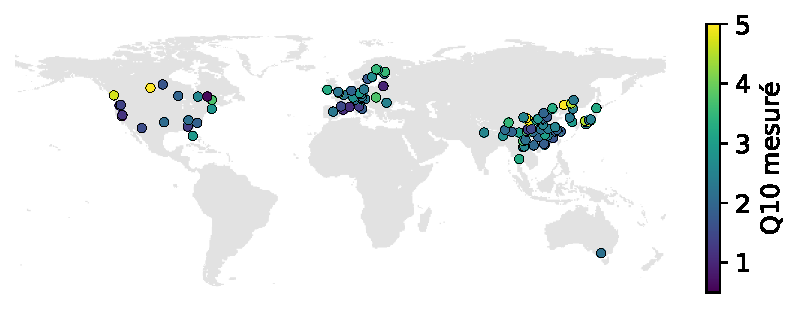
\includegraphics[width=\linewidth]{sites}
    \column{0.38\textwidth}
      \small
      \begin{itemize}
        \item 173 mesures, regroupées en \textbf{131 sites}.
        \item \textbf{99 \%} dans l'hémisphère Nord, \textbf{58 \%} en Asie de l'Est, \textbf{aucun} en Afrique ni en Amérique du Sud.
        \item \textbf{Bruit local} : sur un même site, l'écart-type du \Qdix{} vaut déjà 0.45 (contre 0.96 au total). Même avec des variables parfaites, $R^2 \le 0.78$.
      \end{itemize}
  \end{columns}
  \retenir{notre échantillon ne représente pas la planète : c'est la limite principale de tout le projet.}
\end{frame}

\begin{frame}{Juger un modèle sur des régions qu'il n'a jamais vues}
  \begin{columns}[c]
    \column{0.6\textwidth}
      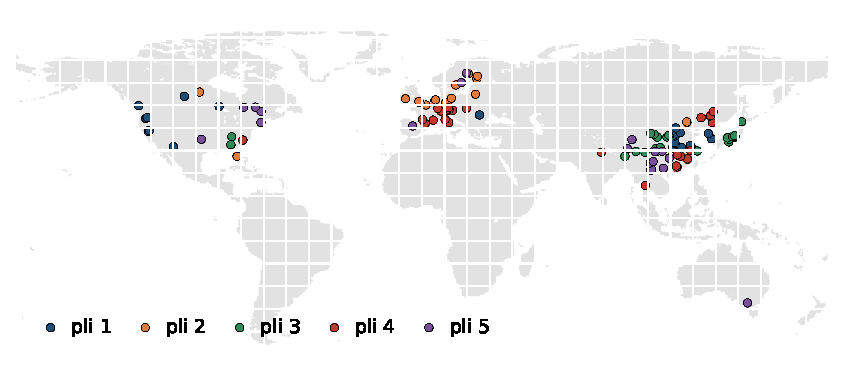
\includegraphics[width=\linewidth]{zones_spatiales}
    \column{0.38\textwidth}
      \small
      \begin{itemize}
        \item Des sites distants de moins de $\approx$ 1\,500 km se ressemblent. Tester sur des sites tirés au hasard mesure en partie de la \textbf{mémoire}.
        \item On retire donc des \textbf{zones entières} de $10^\circ \times 10^\circ$ : 5 plis, répétés 20 fois, soit 100 évaluations, les mêmes pour tous les modèles.
        \item \textbf{Règle fixée à l'avance} : on retient le modèle le plus simple parmi ceux qui ne se distinguent pas du meilleur.
      \end{itemize}
  \end{columns}
  \retenir{un modèle n'est jugé meilleur qu'un autre qu'avec $\approx$ 0.02 à 0.06 de RMSE d'avance : en dessous, c'est du bruit.}
\end{frame}

% =====================================================================
\section{Résultats}

\begin{frame}{Un signal robuste, mais faible}
  \begin{columns}[c]
    \column{0.5\textwidth}
      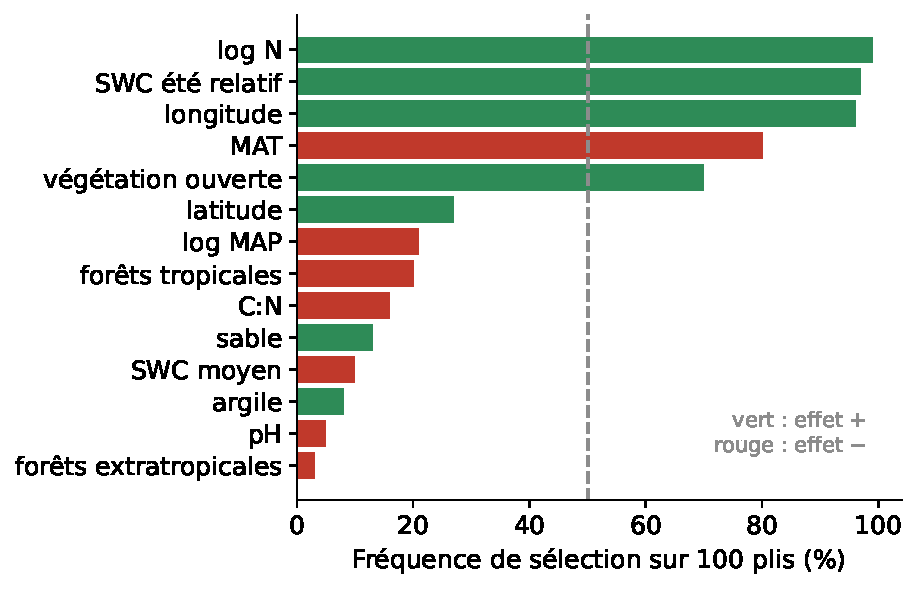
\includegraphics[width=\linewidth]{lasso_stabilite}
    \column{0.48\textwidth}
      \small
      \begin{itemize}
        \item Sélection LASSO refaite sur les 100 plis. \textbf{Cinq variables} reviennent dans au moins 70 \% des plis, toujours avec le même signe : azote ($+$), humidité estivale ($+$), longitude ($+$), MAT ($-$), végétation ouverte ($+$).
        \item \textbf{Le pH}, central chez Hacopian, n'est retenu que dans 5 \% des plis.
        \item Les sites méditerranéens ont le \Qdix{} le plus bas (1.27) \textbf{et} l'été le plus sec.
        \item Signal faible : avec une règle de sélection prudente, \textbf{aucune variable} n'est retenue dans 66 \% des plis.
      \end{itemize}
  \end{columns}
  \retenir{nouveau par rapport à Hacopian : l'azote et la sécheresse estivale, qui semble freiner la réponse des microbes à la chaleur.}
\end{frame}

\begin{frame}{Battre 2.0 est facile ; battre la moyenne, beaucoup moins}
  \begin{columns}[c]
    \column{0.52\textwidth}
      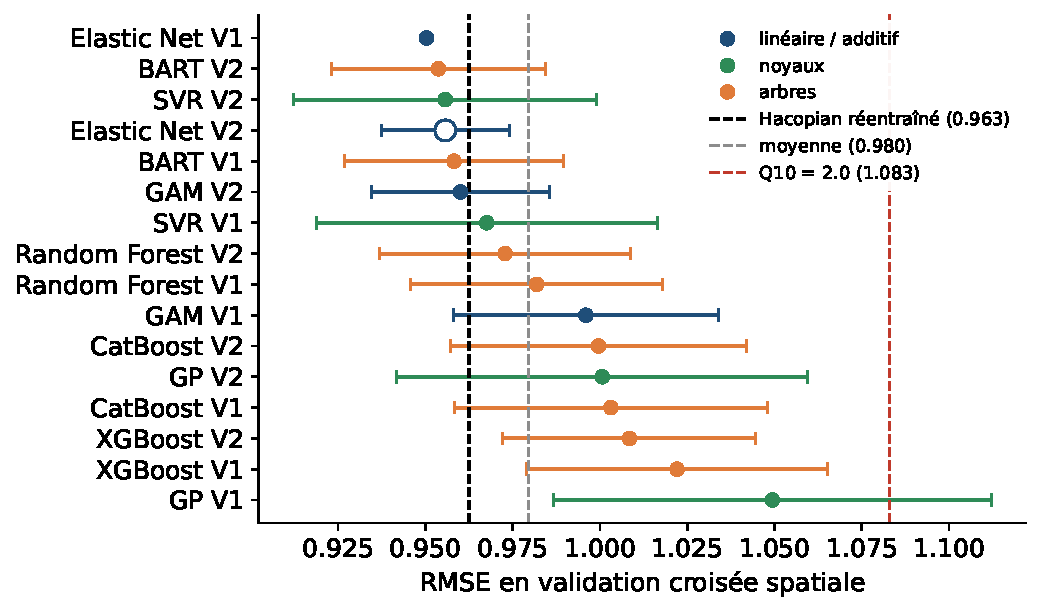
\includegraphics[width=\linewidth]{comparaison_modeles}
    \column{0.46\textwidth}
      \small
      Modèle retenu (Elastic Net) face aux références :

      \vspace{0.1cm}
      \footnotesize\setlength{\tabcolsep}{4pt}
      \begin{tabular}{@{}lcc@{}}
        \toprule
        contre & écart RMSE & plis gagnés \\
        \midrule
        $\Qdix=2.0$ & $-0.127 \pm 0.056$ & 92 \% \\
        moyenne des sites & $-0.024 \pm 0.059$ & 66 \% \\
        Hacopian réentraîné & $-0.007 \pm 0.062$ & 58 \% \\
        \bottomrule
      \end{tabular}
      \small
      \begin{itemize}
        \item Gain de 12 \% sur 2.0, dont \textbf{9.5 points} viennent du seul niveau moyen (2.51 sur nos sites).
        \item L'équation publiée de Hacopian bat 2.0 sur ses 70 sites d'origine, mais \textbf{pas sur les 61 autres}.
      \end{itemize}
  \end{columns}
  \retenir{battre 2.0 : oui. Prédire les différences de \Qdix{} d'une région à l'autre : très peu, avec ces données.}
\end{frame}

\begin{frame}{Expliquer ces sites n'est pas prédire une région}
  \begin{columns}[c]
    \column{0.55\textwidth}
      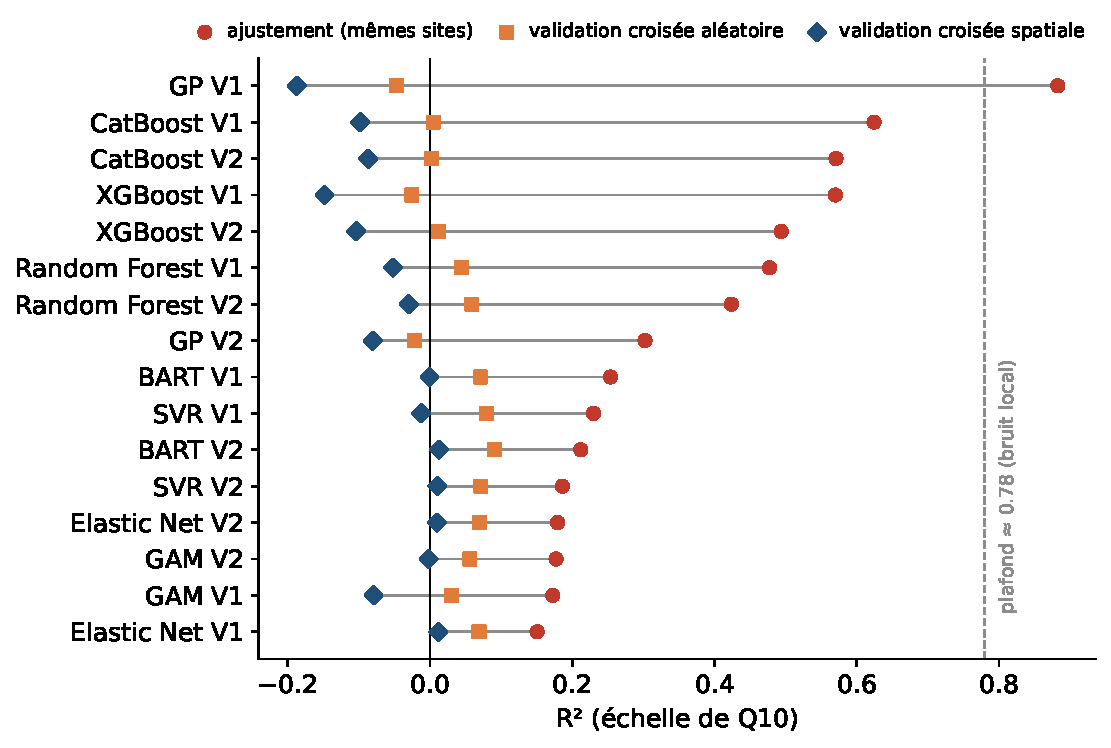
\includegraphics[width=\linewidth]{r2_trois}
    \column{0.43\textwidth}
      \small
      \begin{itemize}
        \item 8 modèles, du linéaire au boosting : \textbf{10 configurations sur 16} sont équivalentes.
        \item Sur leurs propres sites, les plus flexibles atteignent $R^2 = 0.88$, au-dessus du plafond de 0.78 : ils apprennent le bruit par cœur.
        \item Sur des régions nouvelles : $R^2 \le 0.013$ pour tous, \textbf{négatif} pour les plus flexibles.
        \item Choix : \textbf{Elastic Net}, le plus simple des modèles équivalents.
      \end{itemize}
  \end{columns}
  \retenir{plus un modèle explique ses propres sites, moins il prédit les régions nouvelles : avec 131 sites, la complexité ne paie pas.}
\end{frame}

\begin{frame}{Des sites synthétiques ne remplacent pas de vraies mesures}
  \begin{columns}[t]
    \column{0.48\textwidth}
      \small
      \textbf{Le test} : compenser le manque de sites en en fabriquant.
      \begin{enumerate}
        \item Dans chaque pli, une \textbf{copule gaussienne} apprend la loi jointe des sites d'entraînement (variables, \Qdix{} et leurs dépendances).
        \item On en tire 131 ou 1\,000 sites \textbf{synthétiques}, ajoutés à l'entraînement.
        \item Évaluation sur les mêmes zones retirées.
      \end{enumerate}
      \textbf{Fidélité} : un classifieur ne sépare qu'en partie vrais et faux sites (AUC 0.69, contre 0.86 sans les dépendances). Mais les valeurs sont recombinées à partir des nôtres : 56 \% des synthétiques en Asie de l'Est, 58 \% des vrais.
    \column{0.48\textwidth}
      \small
      \textbf{Les résultats} (RMSE en régions nouvelles) :

      \vspace{0.1cm}
      \begin{tabular}{lcc}
        \toprule
        Entraînement & Ridge & Forêt \\
        \midrule
        sites réels & \textbf{0.933} & 1.000 \\
        $+$ 131 synthétiques & 0.954 & 0.988 \\
        $+$ 1\,000 synthétiques & 0.973 & 0.971 \\
        \bottomrule
      \end{tabular}
      \begin{itemize}
        \item \textbf{Ridge} : se dégrade, car les faux sites faussent le réglage de sa pénalité. À pénalité égale : aucun effet ($+0.004 \pm 0.012$).
        \item \textbf{Forêt} : léger mieux, sous une erreur standard : un simple effet de régularisation.
        \item Avec 1\,000 synthétiques, les deux convergent vers $\approx 0.97$ : la relation apprise par la copule.
      \end{itemize}
  \end{columns}
  \retenir{résultat attendu et confirmé : un générateur ajusté sur nos sites n'en sait pas plus qu'eux. Piste écartée ; les copules restent utiles pour des études de simulation.}
\end{frame}

\begin{frame}{Ce que les variables n'expliquent pas}
  \begin{columns}[c]
    \column{0.55\textwidth}
      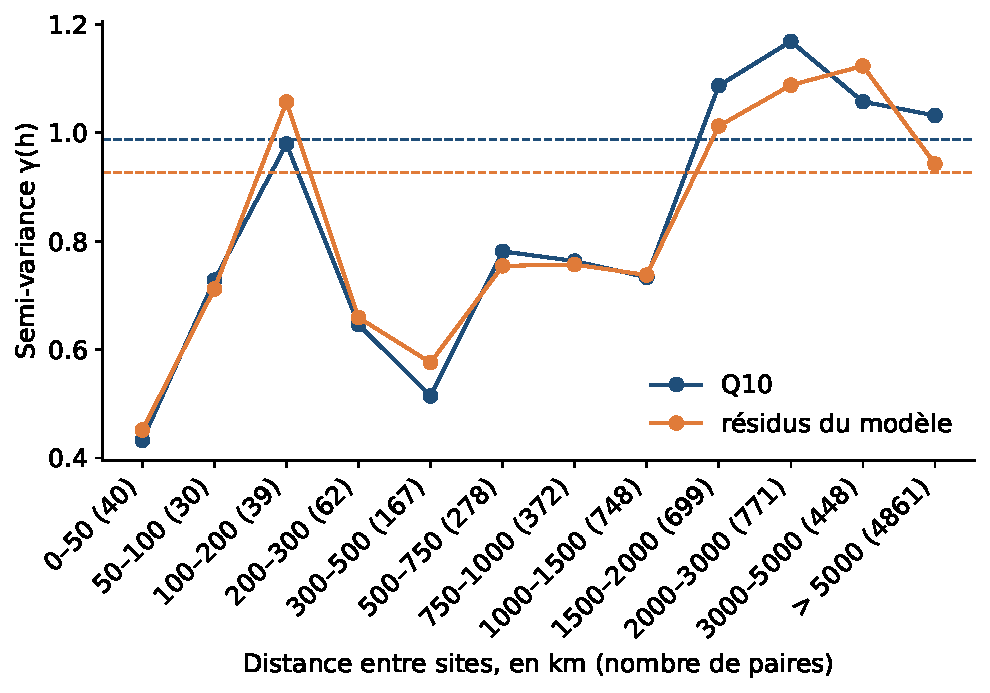
\includegraphics[width=\linewidth]{variogramme_residus}
    \column{0.43\textwidth}
      \small
      \begin{itemize}
        \item Les \textbf{erreurs} du modèle se ressemblent entre sites voisins presque autant que le \Qdix{} lui-même.
        \item Cette ressemblance, jusqu'à $\approx$ 1\,500 km, ne vient donc ni du climat ni du sol.
        \item Pistes : communautés microbiennes, méthodes de mesure propres à une région\dots
      \end{itemize}
  \end{columns}
  \retenir{une information spatiale reste exploitable (krigeage des résidus), mais seulement près de nos sites.}
\end{frame}

% =====================================================================
\section{Vers la carte mondiale}

\begin{frame}{La carte extrapole sur près des deux tiers des terres}
  \begin{columns}[c]
    \column{0.6\textwidth}
      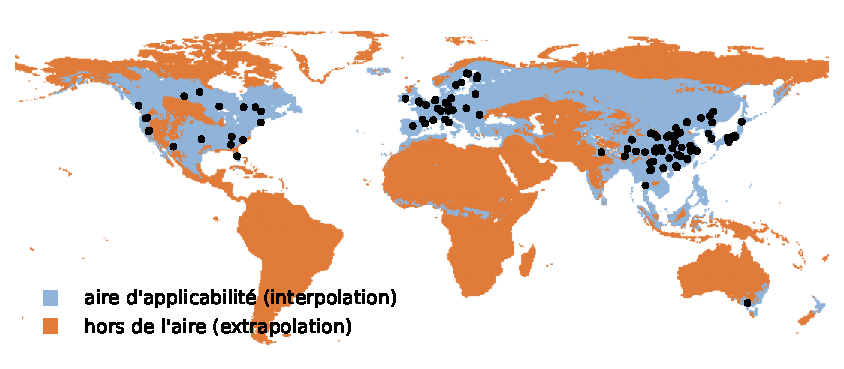
\includegraphics[width=\linewidth]{aire_applicabilite}
    \column{0.38\textwidth}
      \small
      \begin{itemize}
        \item Grille mondiale de $0.5^\circ$, mêmes sources qu'à l'entraînement : concordance aux sites de 0.92 à 0.99.
        \item MAT de nos sites : $-5.2$ à $24.5$ °C ; sur la grille : $-22.2$ à $33.5$ °C.
        \item Seulement \textbf{36 \% des terres} sont dans l'aire d'applicabilité du modèle.
      \end{itemize}
  \end{columns}
  \retenir{l'Amérique du Sud, l'Afrique, l'Australie intérieure, l'Arctique et la Sibérie sont des extrapolations.}
\end{frame}

\begin{frame}{Là où le choix du modèle compte}
  \centering
  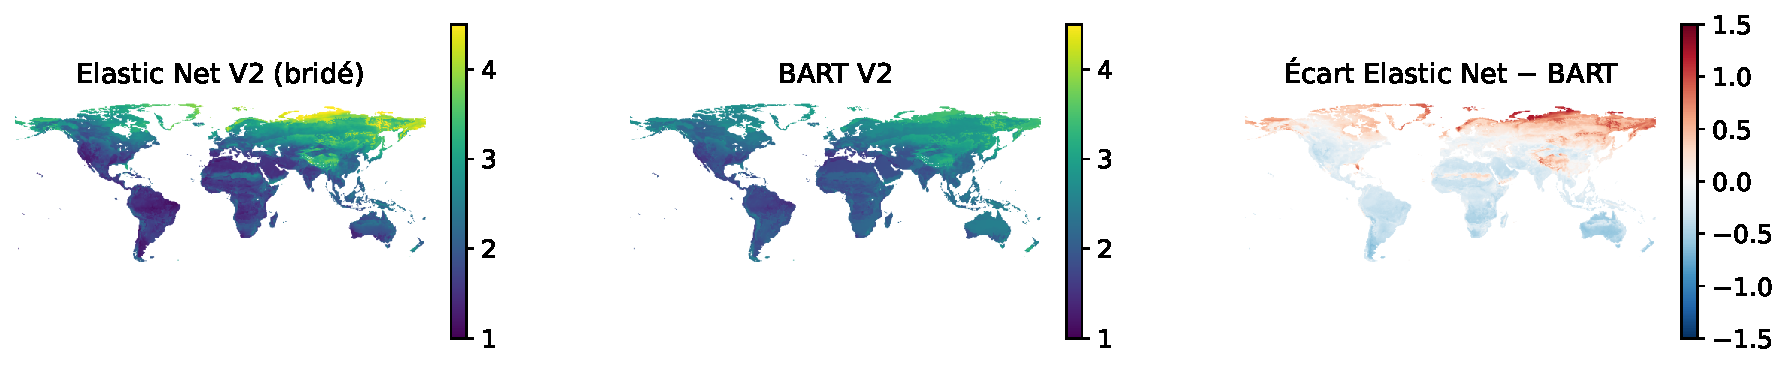
\includegraphics[width=\linewidth]{cartes_modeles}
  \small
  \begin{columns}[t]
    \column{0.5\textwidth}
      \begin{itemize}
        \item \textbf{Près de nos sites}, les modèles s'accordent ($\Qdix \approx 2.4$).
        \item \textbf{Moyenne mondiale} : 2.1 à 2.2, proche de 2.0.
      \end{itemize}
    \column{0.48\textwidth}
      \begin{itemize}
        \item \textbf{Régions froides} (10 \% des terres, aucun site) : de 2.82 à 3.40 selon le modèle.
      \end{itemize}
  \end{columns}
  \retenir{la carte apporte surtout une \textbf{répartition} du \Qdix{} ; l'incertitude est maximale là où se trouve le permafrost.}
\end{frame}

% =====================================================================
\section{Bilan et suite}

\begin{frame}{Nos hypothèses, confrontées aux résultats}
  \small
  \begin{tabular}{p{0.42\textwidth}p{0.5\textwidth}}
    \toprule
    Hypothèse & Verdict \\
    \midrule
    \Qdix{} prévisible depuis des cartes & \textbf{en partie} : signal robuste mais faible ($R^2\approx0$ en régions nouvelles) \\
    Plus de variables aident & \textbf{en partie} : azote et humidité estivale entrent ; le pH sort \\
    Le ML flexible bat le linéaire & \textcolor{rouge}{\textbf{non}} : il apprend le bruit, le linéaire reste en tête \\
    Des données synthétiques compensent le manque de sites & \textcolor{rouge}{\textbf{non}} : un générateur ajusté sur nos sites n'apporte aucune information nouvelle \\
    Les coordonnées sont utiles & \textbf{oui pour la longitude} (effet Asie de l'Est) ; origine à éclaircir \\
    Le biome est un bon prédicteur & \textbf{indécidable} : notre test ne détecterait un effet réel que 2 fois sur 3 \\
    \bottomrule
  \end{tabular}
  \retenir{le facteur limitant n'est pas le modèle, mais la couverture géographique des données.}
\end{frame}

\begin{frame}{Proposition : un niveau de confiance et une valeur de repli}
  \begin{columns}[c]
    \column{0.6\textwidth}
      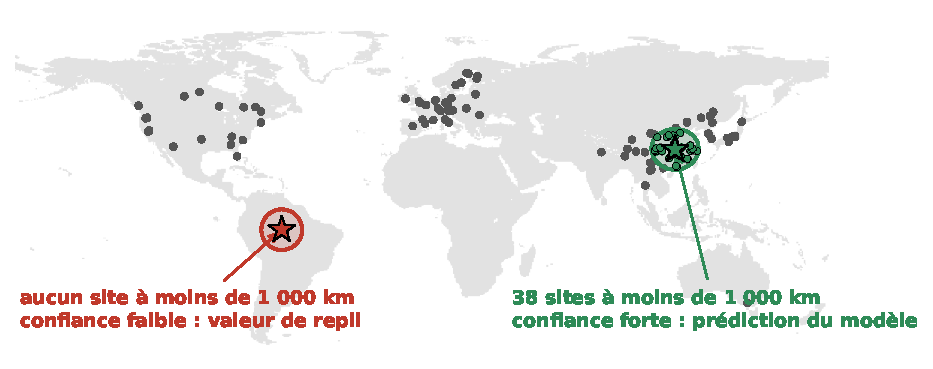
\includegraphics[width=\linewidth]{confiance}
    \column{0.38\textwidth}
      \small
      \begin{itemize}
        \item \textbf{Confiance} : $c(x)=\min\big(1,\,n_r(x)/n^*\big)$, où $n_r(x)$ est le nombre de sites à moins de $r\approx 1\,000$ km.
        \item \textbf{Règle} : prédiction du modèle si $c(x)\ge\alpha$, sinon \textbf{valeur de repli} (2.0, ou une valeur propre à la zone).
        \item \textbf{Sans saut} : $c\,\hat f + (1-c)\,\Qdix^{\text{repli}}$.
        \item \textbf{Aujourd'hui} : 30 \% des terres ont au moins un site à moins de 1\,000 km ; 13 \% en ont au moins cinq.
      \end{itemize}
  \end{columns}
  \retenir{la carte prédirait là où elle dispose d'informations, et reviendrait à une valeur prudente ailleurs.}
\end{frame}

\begin{frame}{Pour la suite}
  \begin{columns}[t]
    \column{0.32\textwidth}
      \textbf{\color{bleu}Données}
      \small
      \begin{itemize}
        \item \textbf{Ajouter des sites} dans les régions froides et tropicales : le levier le plus puissant.
        \item Végétation réelle (MODIS, PFT d'ORCHIDEE) à la place du biome.
      \end{itemize}
    \column{0.32\textwidth}
      \textbf{\color{bleu}Méthodes}
      \small
      \begin{itemize}
        \item Krigeage des résidus, près des sites.
        \item Modèle hiérarchique par classe de végétation.
        \item Carte d'incertitude : intervalles du BART et aire d'applicabilité.
      \end{itemize}
    \column{0.32\textwidth}
      \textbf{\color{bleu}Au-delà}
      \small
      \begin{itemize}
        \item \Qdix{} dynamique : $\Qdix = f(\text{climat})$, utilisable dans les scénarios.
        \item Modèle MMRT, qui décrit mieux la réponse à la température.
      \end{itemize}
  \end{columns}
  \retenir{la carte actuelle bat 2.0 ; la rendre fiable partout demande surtout de nouvelles mesures là où il n'y en a pas.}
\end{frame}

\end{document}
